\documentclass[12pt]{article}
\usepackage{amsmath}
\usepackage{graphicx}
\usepackage{hyperref}
\usepackage{geometry}
\usepackage{booktabs} % for nice tables
\geometry{margin=1in}

\title{Problem Set 4}
\author{Ayse}
\date{\today}

\begin{document}

\maketitle

\section*{Data and Sample Selection}

The data come from the \texttt{PSID} (Panel Study of Income Dynamics).  
We construct the hourly wage as labor income divided by annual hours worked.  
The following restrictions are applied to the sample:
\begin{itemize}
  \item Male heads of household only.
  \item Age between 25 and 60 years.
  \item Hourly wage greater than \$7.
\end{itemize}

The dependent variable in all regressions is the log of the hourly wage.  
Key regressors include years of schooling (\texttt{educ}), age and age squared, and indicator variables for race/ethnicity (Black, Hispanic, and Other).

\section*{Likelihood Function}


We estimate the following log-wage regression model:
\[
\ln(w_{it}) 
= \beta_0 
+ \beta_1 \text{Educ}_{it} 
+ \beta_2 \text{Age}_{it} 
+ \beta_3 \text{Age}^2_{it} 
+ \beta_4 \text{Black}_{it} 
+ \beta_5 \text{Hispanic}_{it} 
+ \beta_6 \text{OtherRace}_{it} 
+ \varepsilon_{it},
\]
where $\varepsilon_{it} \sim \mathcal{N}(0, \sigma^2)$.

\bigskip


The likelihood function for parameters $\beta$ and $\sigma$ is:
\[
L(\beta, \sigma \mid y, X) 
= \prod_{i=1}^n \frac{1}{\sqrt{2 \pi \sigma^2}} 
  \exp\!\left( -\frac{(y_i - X_i \beta)^2}{2\sigma^2} \right).
\]

Taking logs, the log-likelihood is:
\[
\ell(\beta, \sigma \mid y, X) 
= -\frac{n}{2}\ln(2\pi\sigma^2) 
  - \frac{1}{2\sigma^2}\sum_{i=1}^n (y_i - X_i \beta)^2.
\]

The negative log-likelihood (minimized during estimation) is simply
\[
-\ell(\beta, \sigma \mid y, X).
\]


\section*{Results and Interpretation}

Table~\ref{tab:ols-mle} compares the OLS and MLE estimates of the education coefficient ($\beta_1$) across selected years.

\begin{table}[h!]
\centering
\begin{tabular}{@{}lcc@{}}
\toprule
Year & OLS $\hat{\beta}_1$ & MLE $\hat{\beta}_1$ \\
\midrule
1971 & 0.067 & 0.067 \\
1980 & 0.066 & 0.066 \\
1990 & 0.096 & 0.096 \\
2000 & 0.110 & 0.110 \\
\bottomrule
\end{tabular}
\caption{Comparison of OLS and MLE estimates of the education coefficient.}
\label{tab:ols-mle}
\end{table}

The coefficient on education ($\beta_1$) measures the approximate percentage increase in hourly wages associated with an additional year of schooling. The estimates show:
\begin{itemize}
  \item In 1971, returns to schooling were about 6.7\%.
  \item In 1980, they remained roughly constant at 6.6\%.
  \item By 1990, they rose to about 9.6\%.
  \item By 2000, they further increased to around 11.0\%.
\end{itemize}

Overall, these results indicate that returns to education were stable during the 1970s and 1980s but increased substantially in the 1990s and 2000s, suggesting that education became increasingly rewarded in the labor market.
\newpage


\section*{Unit Test}

Figure~\ref{fig:pytest} shows a screenshot of successful test results when running \texttt{pytest} in the terminal.

\begin{figure}[h!]
    \centering
    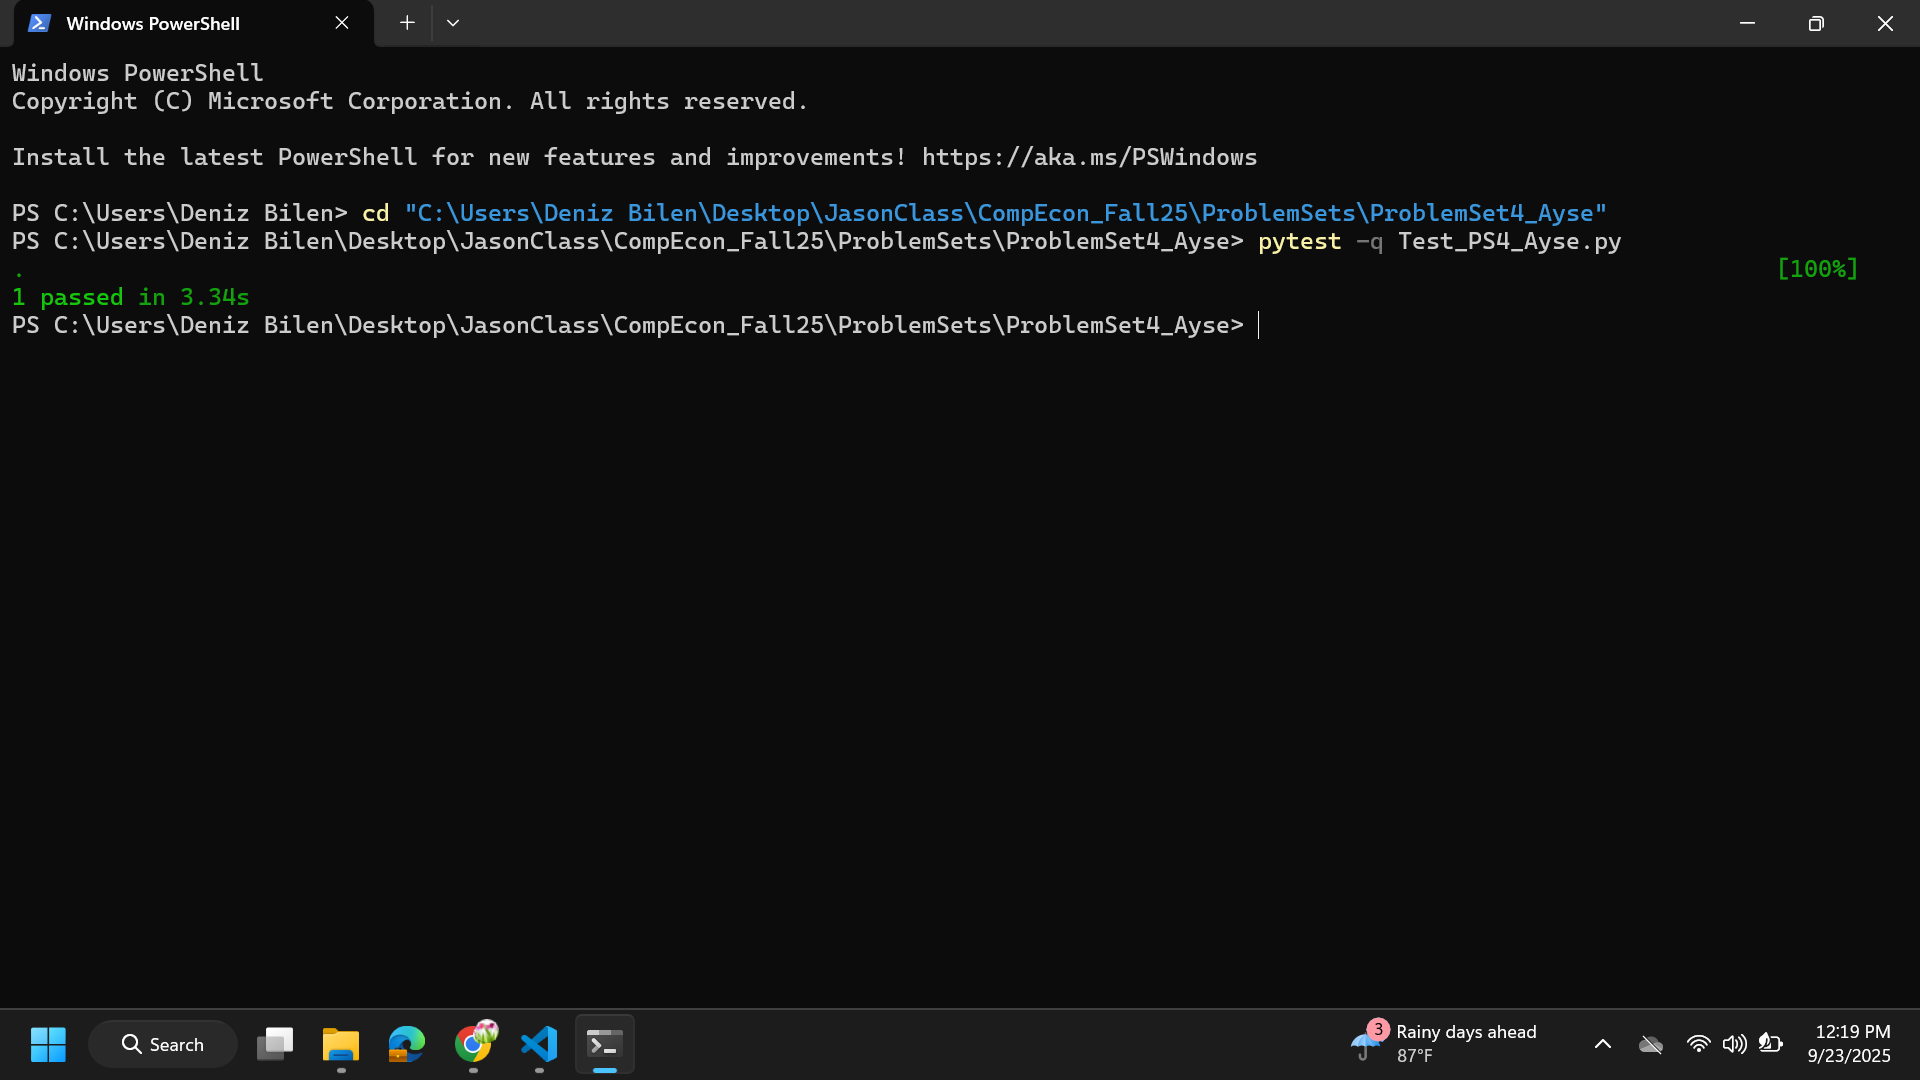
\includegraphics[width=0.9\textwidth]{Test_ScreenShot_Ayse.png}
    \caption{Successful \texttt{pytest} run for unit tests.}
    \label{fig:pytest}
\end{figure}

\end{document}
